\documentclass{article}
\usepackage[UTF8]{ctex}
\usepackage{geometry}
\usepackage{natbib}
\geometry{left=3.18cm,right=3.18cm,top=2.54cm,bottom=2.54cm}
\usepackage{graphicx}
\pagestyle{plain}	
\usepackage{setspace}
\usepackage{caption2}
\usepackage{datetime} %日期
\renewcommand{\today}{\number\year 年 \number\month 月 \number\day 日}
\renewcommand{\captionlabelfont}{\small}
\renewcommand{\captionfont}{\small}
\begin{document}

\begin{figure}
    \centering
    
\includegraphics[width=8cm]{upc.png}

    \label{figupc}
\end{figure}

	\begin{center}
		\quad \\
		\quad \\
		\heiti \fontsize{45}{17} \quad \quad \quad 
		\vskip 1.5cm
		\heiti \zihao{2} 《计算科学导论》课程总结报告
	\end{center}
	\vskip 2.0cm
		
	\begin{quotation}
% 	\begin{center}
		\doublespacing
		
        \zihao{4}\par\setlength\parindent{7em}
		\quad 

		学生姓名:\underline{\qquad  王烁 \qquad \qquad}

		学\hspace{0.61cm} 号:\underline{\qquad 1907010212\qquad}
		
		专业班级:\underline{\qquad 本研人工智能  \qquad  }
		
        学\hspace{0.61cm} 院:\underline{计算机科学与技术学院}
% 	\end{center}
		\vskip 2cm
		\centering
		\begin{table}[h]
            \centering 
            \zihao{4}
            \begin{tabular}{|c|c|c|c|c|c|c|}
            % 这里的rl 与表格对应可以看到,姓名是r,右对齐的;学号是l,左对齐的;若想居中,使用c关键字。
                \hline
                课程认识 & 问题思 考 & 格式规范  & IT工具  & Latex附加  & 总分 & 评阅教师 \\
                30\% & 30\% & 20\% & 20\% & 10\% &  &  \\
                \hline
                 & & & & & &\\
                & & & & & &\\
                \hline
            \end{tabular}
        \end{table}
		\vskip 2cm
		\today
	\end{quotation}

\thispagestyle{empty}
\newpage
\setcounter{page}{1}
% 在这之前是封面,在这之后是正文
\section{引言}
随着信息时代的不断发展,各行各业发展越来越智能化,信息化,计算机的应用也变得必不可缺。人们可以通过计算机处理大量的数据,提高工作效率,可以通过利用计算机设计新的结构模型,解决无法验证的问题。准确的来说,人类不断改进计算机的同时,计算机也在不断改变人们的生活。计算机技术应用的发展是各国努力实现的创新成果之一,也是人类社会进步与否最直接的表现,只有计算机技术的大力发展,才能更好的衔接各个领域技术的进步。对于我们来说,较为全面准确的把握计算机科学与技术领域各个知识的相互联系,构造较为完善的知识网络体系,确定未来的发展方向,是最基本也是最重要的事情。\par
《计算科学导论》重在引导学生怎么从科学哲学的角度去认识和学习计算科学,有助于学生正确理解计算科学,学好计算机技术,顺利完成学业任务,对我们个人来说具有极大帮助与重要意义。

\section{对计算科学导论这门课程的认识、体会}
计算科学导论属于学科入门性导引课程,使用教材为赵致琢所著《计算科学导论》,孙老师通过雨课堂讲授与引导我们进行主题演讲、讨论,来讲述本门课程,通过对计算学科基本知识和学科方法论方面知识来培养我们对计算领域热点的兴趣,从而帮助我们确立完善个人职业规划,明白未来研究发展方向。\par
本学科基本概念:计算模型,二进制,通用数字计算机系统结构与工作原理,数字逻辑与集成电路,机器指令与汇编语言,算法,过程与程序,高级语言与程序设计,程序设计方法与技术,系统软件与应用软件,计算机图形学,图像处理与模式识别,逻辑与人工智能,计算机组织与系统结构,通道与并行计算,计算机网络与通信,高性能计算;\par
学科的定义、范畴、范型、意义、内容和方法:学科的定义,基本问题,发展主线,主流方向,学科形态,核心概念,历史渊源,发展变化,典型方法,典型实例,学科知识组织结构与分类体系,学科基本工作流程方式,学科的逻辑基础,本学科与其他学科的关系;\par
学科教育与教学规律:学科发展的特点和规律,学科发展潮流与未来发展方向,学科人才培养能力体系,培养目标,毕业要求,课程目标,课程体系,各学期重点课程。\par
孙老师通过生动形象的语言,具体详细的实例为我们介绍了各个章节知识,并结合诸如IBM公司发展里程碑事件,图灵测试等许多有意思,充满科学探索意义的故事,帮助我们建\cite{he1}立起了对科学技术学科的兴趣,引起我们对科学技术学科的思索。\par
\subsection{IBM System 360-从计算机到计算机系统}
\begin{figure}[h!]
	\centering
	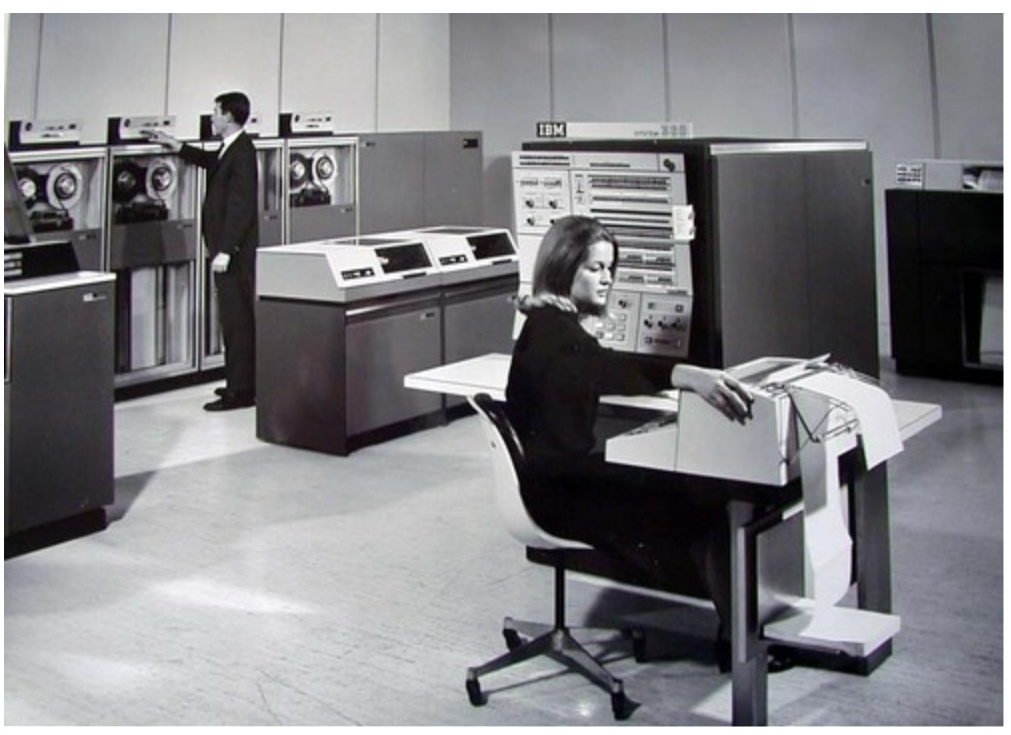
\includegraphics[scale=0.4]{20200103000145}
	\caption{System/360}
	\label{fig:univers}
\end{figure}

1960年,国际商用机器公司(IBM)已成为电脑界的巨头。然而,就在电脑的市场需求日益增长时,IBM却停滞不前。为此,利尔森临危受命,获得动用公司所有资源的权限。经历全面研发和调研后,他决定进行“计算机家族”的研发。
利尔森采取了两个措施,第一,命令电脑事业部调整规划,将现有产品的销售寿命延长到1964年。第二,命令他的核心队伍将“计算机家族”的研究作为第一优先。
到了1961年10月,他的核心队伍仍然对可行性没有一致意见,但认为可行的意见占了上风。利尔森感到必须采取更果断的措施。他从核心队伍中抽出十三名研究人员、技术主管和市场主管,组成了一个特别工作组,限令他们在年底以前必须提出一个计算机家族的总体方案。为了让工作组全力投入,他把工作组全体人员集中到康州的一个旅馆,不拿出方案就别回家。
1961年12月28日,经过工作组两个月的紧张工作,一份题目很不起眼的文档《处理机产品―SPREAD工作组的最后报告》诞生了。这也就是后来赫赫有名的IBM S/360计算机系统的总体方案。
工作组的成员后来领导了S/360系统的设计和工程实施工作。他们中的一些人对计算机技术后来的发展继续发挥重大的影响。工作组组长鲍伯·伊万斯(Bob Evans)后来成了IBM负责技术的副总裁。工作组成员金·阿姆达尔(Gene Amdahl)是计算机体系结构理论中“阿姆达尔定律”的发明者。工作组成员弗利德利克·布鲁克斯(Frederick Brooks)则发现了软件开发的“布鲁克斯定律”。\par
经历了一番曲折探索研发后,IBM Sestem 360 实现了历史性的突破,开创了计算机兼容的时代,创造了世界是第一个通用、最典型的操作系统,实现了基于全硬件虚拟化的虚拟机解决方案,实现了分时的多道程序设计技术。从而一转局势,创造了历史性的突破,一跃成为顶级公司,为世人所知,据统计,这项技术直到今日还在为公司创造收入盈利。\par 
这个真实的故事充满科学哲理:我们想要解决问题,首先,我们必须了解它,了解它的运转体系,现状问题。其次,我们必须制定可行方案,计划合理。接着,我们在必要时需采取果断措施。拖拖拉拉永远完成不了任务,我们得给自己压力,给自己时间期限,不做出来不准停。这样,没有什么解决不了的问题。\par 

\subsection{图灵机}
\begin{figure}[h!]
	\centering
	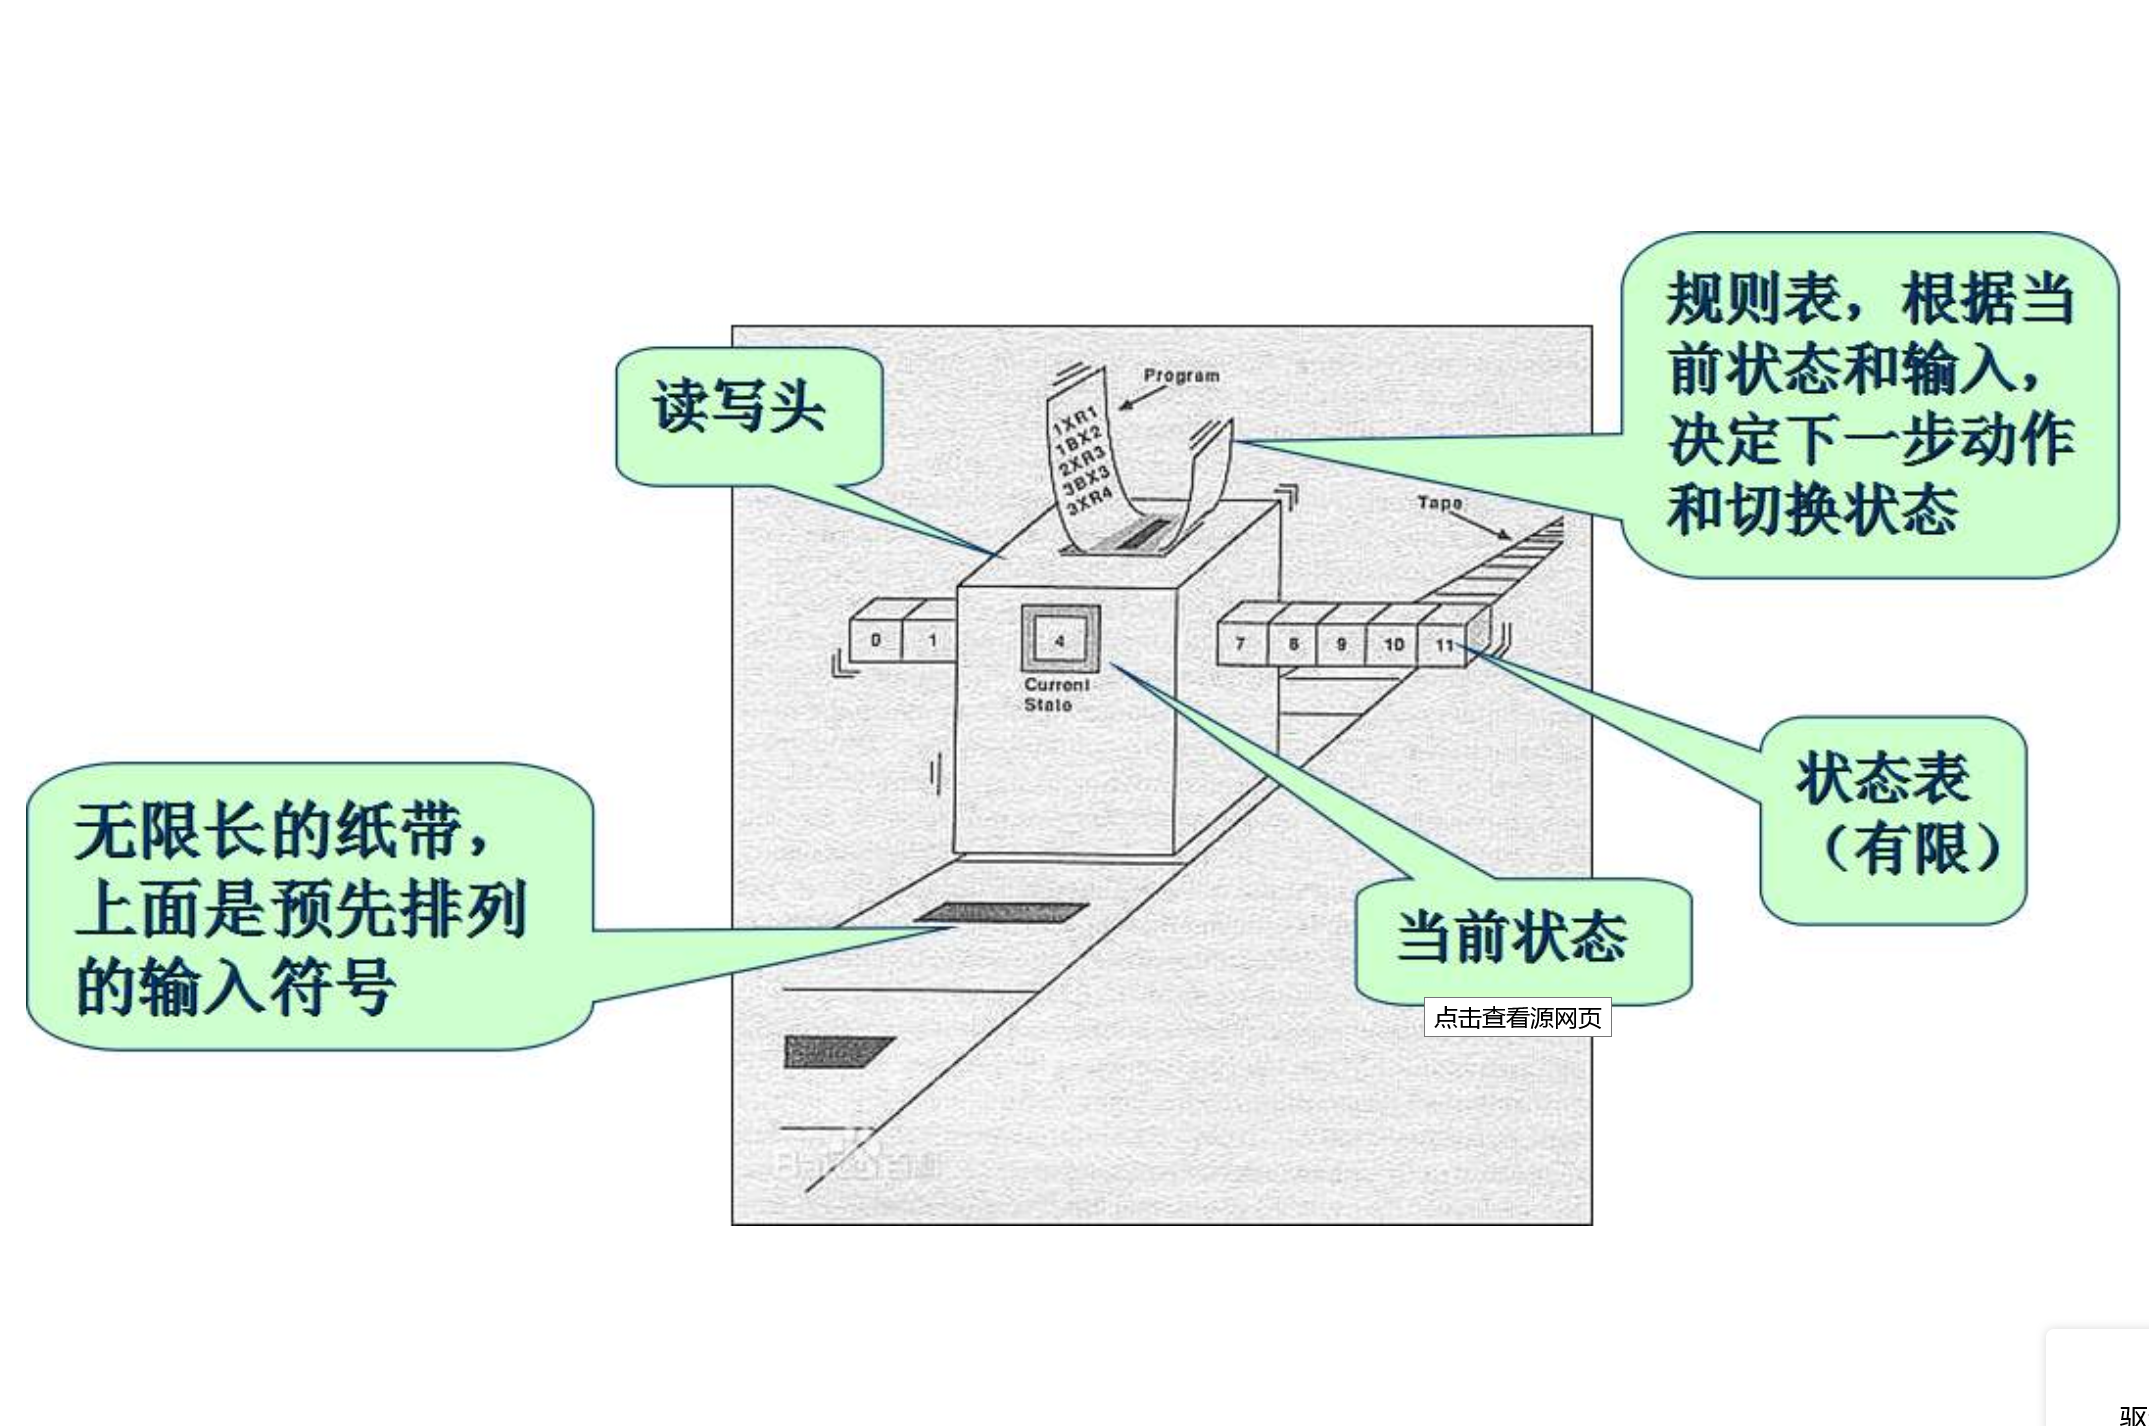
\includegraphics[scale=0.2]{20200103014044}
	\caption{图灵机}
	\label{fig:un}
\end{figure}

所谓的图灵机就是指一个抽象的机器,它有一条无限长的纸带,纸带分成了一个一个的小方格,每个方格有不同的颜色。有一个机器头在纸带上移来移去。机器头有一组内部状态,还有一些固定的程序。在每个时刻,机器头都要从当前纸带上读入一个方格信息,然后结合自己的内部状态查找程序表,根据程序输出信息到纸带方格上\cite{he5},并转换自己的内部状态,然后进行移动。\par 
通常图灵机以一个给定的初始状态和带上的信息开始,然后在状态函数的指导下由一个状态转移到另外一个状态。最后图灵机将处于停机状态。当图灵机到达一个状态函数没有定义的输入时,图灵机将会停止。另外,我们假定对于任意的状态都没有定义其转移函数,图灵机到达状态的时候都会停机。\par 
还有一个著名的实验测试,图灵测试,由艾伦·麦席森·图灵发明,指测试者与被测试者(一个人和一台机器)隔开的情况下,通过一些装置(如键盘)向被测试者随意提问。进行多次测试后,如果机器让平均每个参与者做出超过百分之30的误判,那么这台机器就通过了测试,并被认为具有人类智能。\par 

\section{进一步的思考}
\begin{itemize}
	\item 人工智能是计算机科学的一个分支\cite{he2},它企图了解智能的实质,并生产出一种新的能以人类智能相似的方式做出反应的智能机器,该领域的研究包括机器人、语言识别、图像识别、自然语言处理和专家系统等。人工智能从诞生以来,理论和技术日益成熟,应用领域也不断扩大,可以设想,未来人工智能带来的科技产品,将会是人类智慧的“容器”。人工智能可以对人的意识、思维的信息过程的模拟。人工智能不是人的智能,但能像人那样思考、也可能超过人的智能。人工智能也是一门极富挑战性的科学,从事这项工作的人必须懂得计算机知识,心理学和哲学。人工智能是包括十分广泛的科学,\cite{he3}它由不同的领域组成,如机器学习,计算机视觉等等,总的说来,人工智能研究的一个主要目标是使机器能够胜任一些通常需要人类智能才能完成的复杂工作。但不同的时代、不同的人对这种“复杂工作”的理解是不同的。\par 我对人工智能的感情很早就产生了,早在我是个孩提时,我就喜欢研究机器人玩具。而如今机器人技术更是衡量一个国家人工智能技术最直观的体现。近年来,世界范围内机器人在工业生产设计、医疗诊断操作、复杂危险环境工作、家庭生活便利方面,取得了长足进展和重大突破。谷歌无人汽车、能与真人交流互动的日本机器人pepper、与战机飞行员对抗并获胜的无人驾驶战机等,大大刷新了世人对机器人简单狭隘的认识。今天的机器人,已经不是那种只有一个机械手臂,笨手笨脚、没有交流能力的工具了。而是能独立工作并能与人类一起合作的伙伴了。 
	\item 鉴于我是人工智能本研一体班的学生,对于分组课题演讲的课题,我与队友自然选择了与人工智能方面相关的。我们的课题是——机器仿生。我的队友负责答辩,而我负责演讲。我们主要从三个方面来讨论机器仿生,1、机器仿生的背景与定义;2、研发情况;3、发展前景与趋势。\par 首先,什么是机器仿生?未来的机器人将在人类不能或难以到达的已知或未知环境里为人类工作。人们要求机器人不仅适应原来结构化的、已知的环境,更要适应未来发展中的非结构化的、未知的环境。除了传统的设计方法,人们也把目光对准了生物界,力求从丰富多彩的动植物身上获得灵感,将它们的运动机理和行为方式运用到对机器人运动机理和控制的研究中,这就是仿生学在机器人科学中的应用。这一应用已经成为机器人研究领域的热点之一,势必推动机器人研究的蓬勃发展。而仿生机器人是指模仿自然界中生物的外部形状、运动原理和行为方式的系统,能从事生物特点工作的机器人。仿生机器人分为三类,我们最熟知的仿人机器人、仿生物机器人、生物机器人。模仿人的形态和行为而设计制造的机器人就是仿人机器人,一般分别或同时具有仿人的四肢和头部。仿人机器人研究集机械,电子,计算机,材料,传感器,控制技术等多门科学于一体,代表着一个国家的高科技发展水平。仿人机器人具有人类的外观,可以适应人类的生活和工作环境,代替人类完成各种作业,并可以在很多方面扩展人类的能力,在服务,医疗,教育,娱乐等多个领域得到广泛应用。而仿生物机器人能模仿动物的特性,能够适应不同的环境,活动范围广,躲避风险能力和生存能力强,拥有极强的移动能力,因此能够代替人们到达不可预测的环境中进行各种活动,完成任务。最后,生物机器人是利用单细胞打造成的,具有特殊功能特性的机器人,他们能够完成普通仿真机器人所不能完成的任务,生物机器人被设计成通过光和电磁刺激来激发化学反应。
	生物机器人的最终研究目标是使其具备组装微机器组件的能力。\par
	而在查阅资料的过程中,我们还知道了一个名词——冗余自由度。因为仿生机器人的主要特点就是它们大多为冗余自由度或者是超冗余自由度的机器人,机器结构相对比较复杂。然后我来解释一下什么叫做冗余自由度。冗余顾名思义,就是多余的意思。自由度,按我的理解,通俗来讲就是指一个机器人或者机器手臂中能活动的关节数量,自然而然,冗余自由度越高的机器人就会越灵活。\par
	然后我们来谈谈研发情况,我们先介绍了世界各国的先进成果。日本本田技研工业株式会社研制的智能仿人机器人Asimo,它可以同时与多人进行对话;遭遇其他正在行动中的人时,会预测对方行进方向及速度,自行预先计算替代路线以免与对方相撞。腿部的运动能力及活动范围不仅可以步行、奔跑、倒退走,还可以单脚跳跃、双脚跳跃,更能边跳跃边变换方向,也可以在些微不平的地面行走。它的手部可转开水瓶、握住纸杯、进行倒水,手指动作更纤细,甚至可以边说话边以手语表现说话内容。美国国防高级研究计划局与波士顿动力公司合作研发的BigDog,它能够穿越各种复杂地形,以6.4公里每小时运行,负重150公斤,爬35度的斜坡。它的运动由机载计算机控制,从机器人的各种传感器接收输入,导航和平衡也由控制系统管理。它的行走模式,通过各配备四个低摩擦液压缸执行器的四脚控制。它可以站起来,坐下,一次只抬起一条腿地爬行,只抬起对角线的两条腿地慢跑,或者快速地奔跑。BigDog的移动速度可以在0.2米每秒到1.6米每秒的范围内变化。然后就是我最喜欢,也是最厉害的Atlas了。Atlas是美国波士顿动力公司开发的产品,高约80厘米,重75公斤,它采用电动和液压驱动,身体和腿部安装有先进的传感器以实现平衡,头部使用激光雷达和立体感应器来避开障碍物,评估地形,帮助导航和操纵物体。工程师将将结构,歧管,流体路径和执行器气缸都集成到一个结构中,这使得其具有高强度重量比和极大的工作空间。立体视觉,距离感应和其他传感器使Atlas能够操纵环境中的物体并在崎岖的地形上行走。这些传感器和平衡系统也使得Atlas在受到推挤或推动时能够保持平衡。Atlas的设计初衷是为搜索和救援行动提供紧急服务,执行诸如关闭阀门,打开门以及在人类无法生存的环境中操作动力设备等任务,最终目的是将其应用于最危险和最高风险的工作,例如进入熔毁的核反应堆,关闭深水漏油,制止肆虐野火。
	其实一直以来,世界上都存在反对开发智能机器人的声音。机器人属于新的事物,而人类总是害怕未知的东西。人们希望机器人能够代替人类从事各种劳动,为人类服务,但又担心机器人的发展将引起新的社会问题,甚至威胁到人类的生存。人们在期待中含有几分不安。机器人还可能会导致大量失业。机器人能够代替人类进行各种繁琐的体力劳动和脑力劳动。例如,机器人可以毫无顾忌地冲进火场,所以机器人是天生的消防员;机器人在水下不用担心无法呼吸和水压的问题,所以机器人是天生的潜水员;机器人不怕辛苦,不畏严寒酷暑,所以机器人是天生的清洁工和各种工人之类的例子数不胜数。因此,将有很多工人和技术人员可能把自己的工作让位给机器人,造成他们的下岗和再就业,甚至造成失业。因此我觉得人类应该掌握机器人无法掌握,独一无二的技能,对于机器人的研究应该掌控在我们自己可以管控的范围内。\citep{he4}这是我读过的一篇论文,基于对以后人工智能发展突破点得出的结论。
	\item 在答辩环节,孙老师首先问了我们,机器人存在的伦理问题怎么处理。而我们的回答是,目前世界上智能机器人并没有发展到那种阶段,都是根据编好的程序执行命令的机器人,能具备学习能力和自主能力的机器人可能未来的某一天会出现,但现在是不存在的。就像前那些年吹爆的人工智能机器人,世界上第一个机器人公民——索菲亚,也已经坠落神坛,被证实没有与人交流的能力,只是在执行命令而已。之后,孙老师告诉我们,机器仿生运用最广的地方是军事方面,这也是我们考虑不周的地方。回去之后经过查阅文献得知,军事仿生学是仿生学的一项重要内容,是军事科学和技术的一个极具影响力和生命力的研究领域。它是模仿生物系统的原理和特异功能来发展军事高技术,提高武器装备的性能,发展军事战略技术,提高军队后勤保障的能力。而发展趋势之一的微型机器人,也是军方极力攻坚的一大方向。\par
	
\end{itemize}



\section{总结}
总而言之,对于技术科学导论这门学科我收益良多。它帮助我弄清楚许多原先不懂的名词与概念,让我对技术科学有了整体的把握与理解,也初步对未来的职业规划有了初步计划,同时,与队友合作分工中我也体会到莫大的乐趣与完成任务时的成就感,留下了不可磨灭的印象。懂得许多科学道理。\par
最后,正如孙老师所说:做自己未做过的事;做自己不敢做的事;做自己不愿意做的事。在今后学习工作中,我会谨记老师的教诲,不断提高自己的专业素养,努力奋斗,成为一名高水平人才。

\hspace*{\fill} \\


\bibliographystyle{plain}
\bibliography{references}



\begin{figure}[h!]
	\centering
	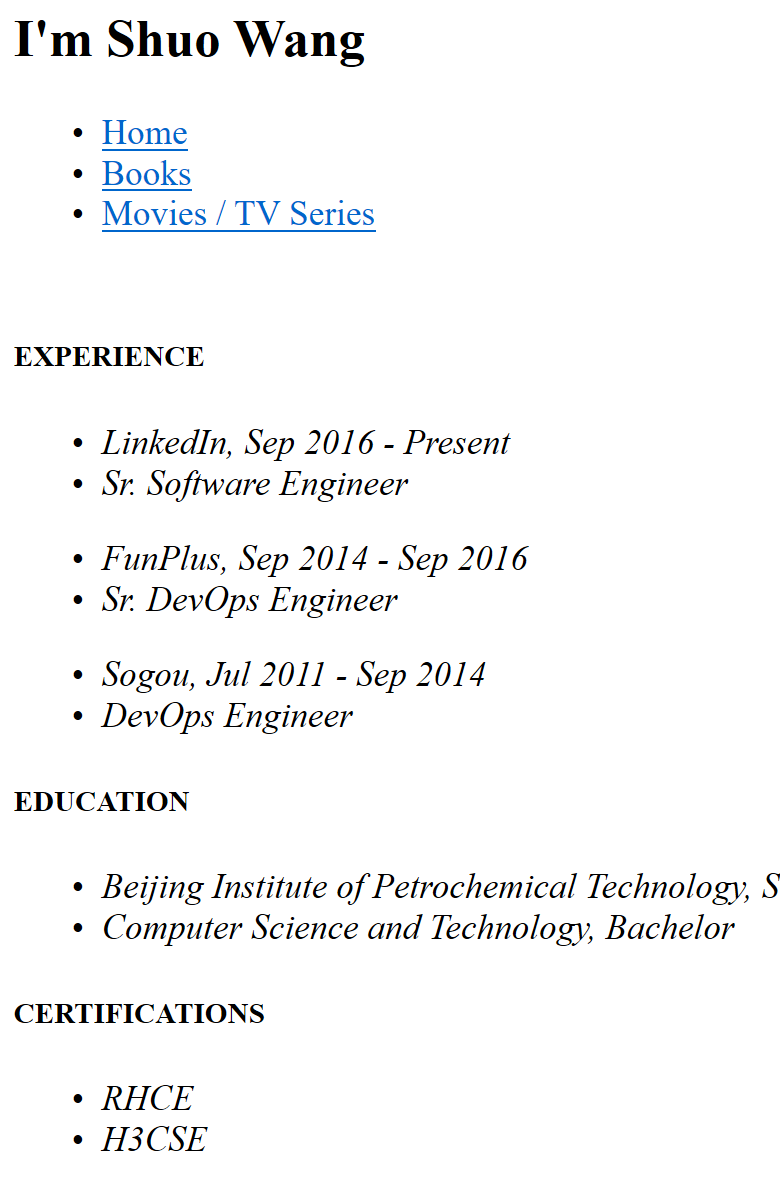
\includegraphics[scale=0.4]{20191127224007}
	\caption{Github个人网站}
	\label{fig:ggrqc.jpg}
\end{figure}


\begin{figure}[h!]
	\centering
	
\includegraphics[scale=0.2]{Screenshot_20191127-132354}
	\caption{观察者截图}
	\label{fig:ggwqc.jpg}
\end{figure}

\begin{figure}[h!]
	\centering
	
\includegraphics[scale=0.2]{Screenshot_20191127-132729}
	\caption{学习强国截图}
	\label{fig:ggwrc.jpg}
\end{figure}

\begin{figure}[h!]
	\centering
	
\includegraphics[scale=0.3]{Screenshot_20191127-224336}
	\caption{b站截图}
	\label{fig:ggwrqc.jpg}
\end{figure}

\begin{figure}[h!]
	\centering
	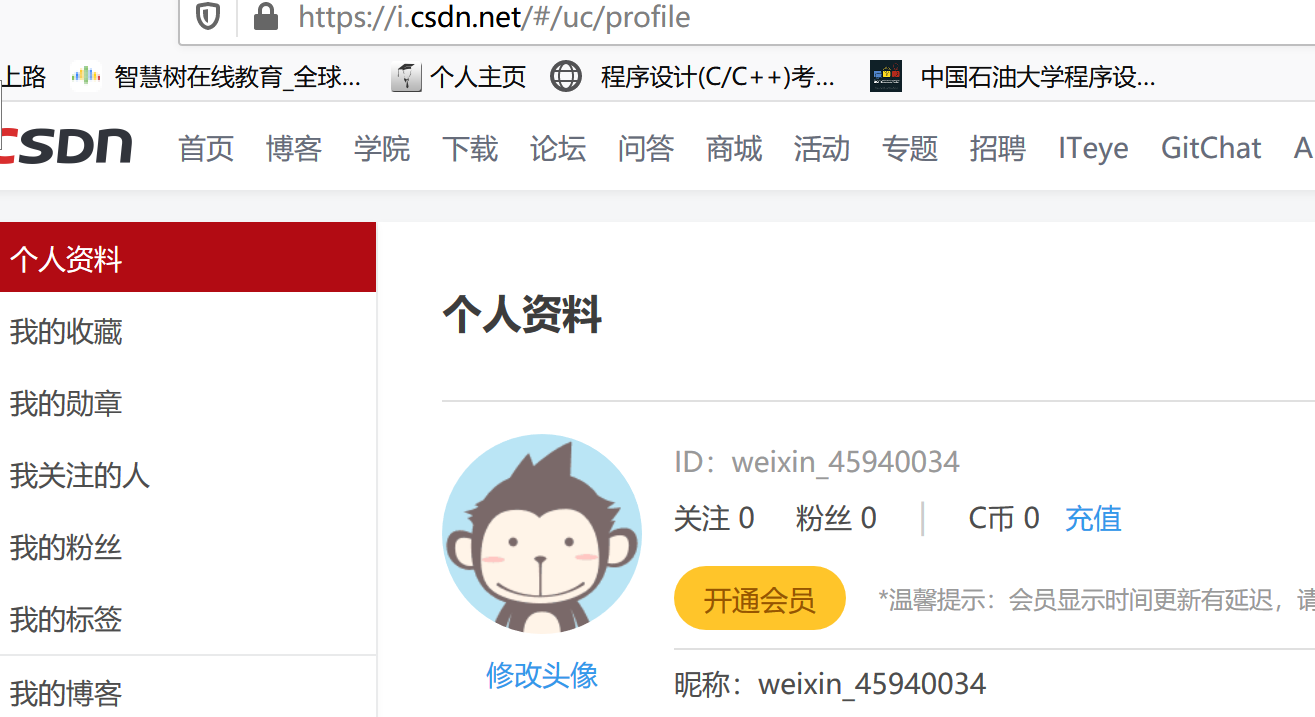
\includegraphics[scale=0.4]{20191127233303}
	\caption{CSDN截图}
	\label{fig:ggwrq.jpg}
\end{figure}

\begin{figure}[h!]
	\centering
	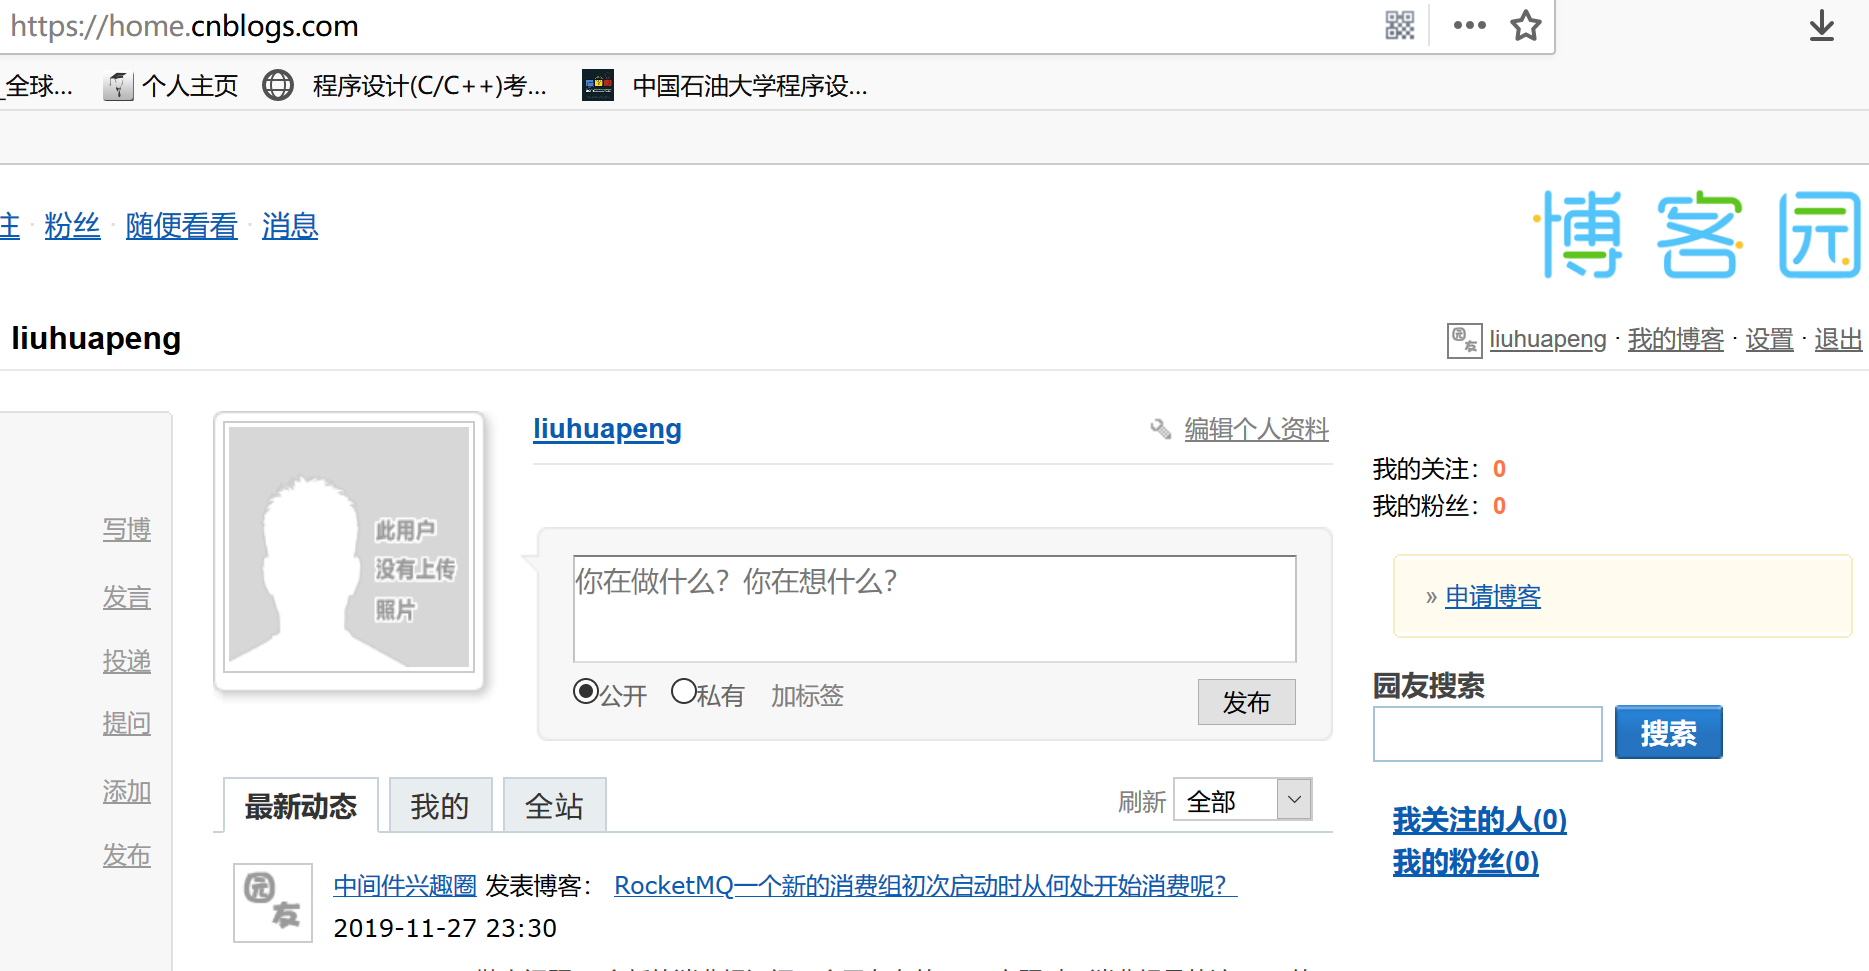
\includegraphics[scale=0.4]{20191127233345}
	\caption{博客园截图}
	\label{fig:ggwrqgc.jpg}
\end{figure}

\begin{figure}[h!]
	\centering
	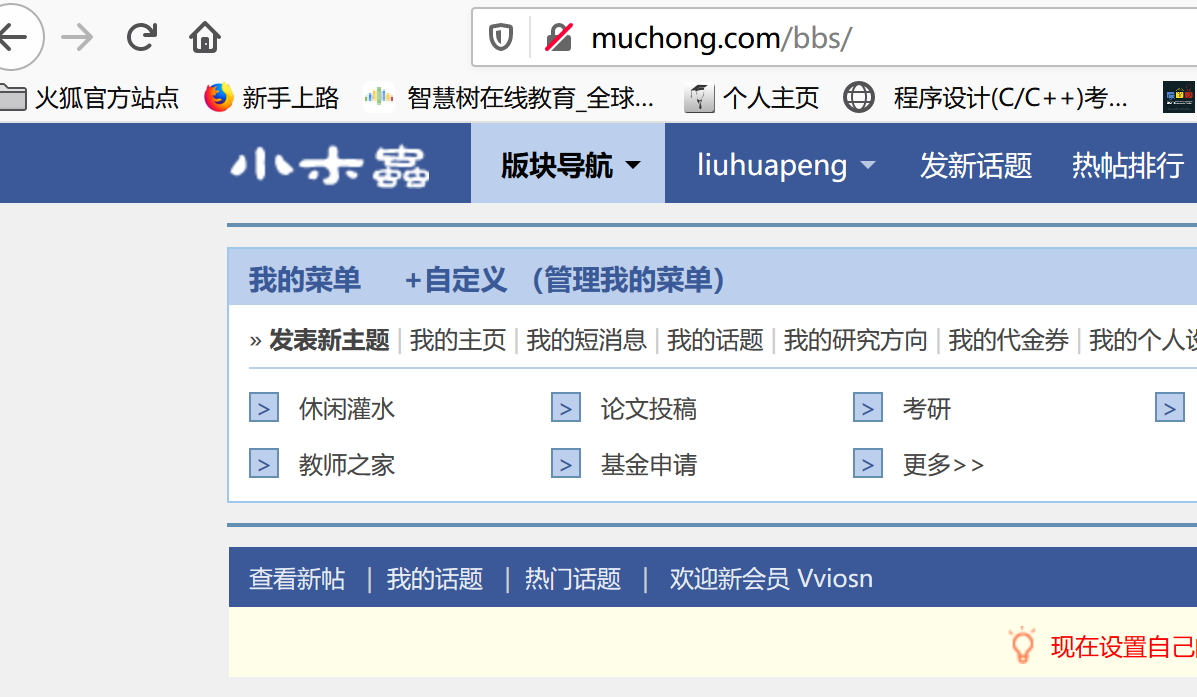
\includegraphics[scale=0.5]{20191128000651}
	\caption{小木虫截图}
	\label{fig:ggwwrqc.jpg}
\end{figure}




\end{document}
